\documentclass[]{article}
\usepackage{lmodern}
\usepackage{amssymb,amsmath}
\usepackage{ifxetex,ifluatex}
\usepackage{fixltx2e} % provides \textsubscript
\ifnum 0\ifxetex 1\fi\ifluatex 1\fi=0 % if pdftex
  \usepackage[T1]{fontenc}
  \usepackage[utf8]{inputenc}
\else % if luatex or xelatex
  \ifxetex
    \usepackage{mathspec}
  \else
    \usepackage{fontspec}
  \fi
  \defaultfontfeatures{Ligatures=TeX,Scale=MatchLowercase}
\fi
% use upquote if available, for straight quotes in verbatim environments
\IfFileExists{upquote.sty}{\usepackage{upquote}}{}
% use microtype if available
\IfFileExists{microtype.sty}{%
\usepackage{microtype}
\UseMicrotypeSet[protrusion]{basicmath} % disable protrusion for tt fonts
}{}
\usepackage[margin=1in]{geometry}
\usepackage{hyperref}
\hypersetup{unicode=true,
            pdftitle={Inferêcia com uso de Intervalo de Confiança},
            pdfauthor={Fabiana Alves},
            pdfborder={0 0 0},
            breaklinks=true}
\urlstyle{same}  % don't use monospace font for urls
\usepackage{color}
\usepackage{fancyvrb}
\newcommand{\VerbBar}{|}
\newcommand{\VERB}{\Verb[commandchars=\\\{\}]}
\DefineVerbatimEnvironment{Highlighting}{Verbatim}{commandchars=\\\{\}}
% Add ',fontsize=\small' for more characters per line
\usepackage{framed}
\definecolor{shadecolor}{RGB}{248,248,248}
\newenvironment{Shaded}{\begin{snugshade}}{\end{snugshade}}
\newcommand{\KeywordTok}[1]{\textcolor[rgb]{0.13,0.29,0.53}{\textbf{#1}}}
\newcommand{\DataTypeTok}[1]{\textcolor[rgb]{0.13,0.29,0.53}{#1}}
\newcommand{\DecValTok}[1]{\textcolor[rgb]{0.00,0.00,0.81}{#1}}
\newcommand{\BaseNTok}[1]{\textcolor[rgb]{0.00,0.00,0.81}{#1}}
\newcommand{\FloatTok}[1]{\textcolor[rgb]{0.00,0.00,0.81}{#1}}
\newcommand{\ConstantTok}[1]{\textcolor[rgb]{0.00,0.00,0.00}{#1}}
\newcommand{\CharTok}[1]{\textcolor[rgb]{0.31,0.60,0.02}{#1}}
\newcommand{\SpecialCharTok}[1]{\textcolor[rgb]{0.00,0.00,0.00}{#1}}
\newcommand{\StringTok}[1]{\textcolor[rgb]{0.31,0.60,0.02}{#1}}
\newcommand{\VerbatimStringTok}[1]{\textcolor[rgb]{0.31,0.60,0.02}{#1}}
\newcommand{\SpecialStringTok}[1]{\textcolor[rgb]{0.31,0.60,0.02}{#1}}
\newcommand{\ImportTok}[1]{#1}
\newcommand{\CommentTok}[1]{\textcolor[rgb]{0.56,0.35,0.01}{\textit{#1}}}
\newcommand{\DocumentationTok}[1]{\textcolor[rgb]{0.56,0.35,0.01}{\textbf{\textit{#1}}}}
\newcommand{\AnnotationTok}[1]{\textcolor[rgb]{0.56,0.35,0.01}{\textbf{\textit{#1}}}}
\newcommand{\CommentVarTok}[1]{\textcolor[rgb]{0.56,0.35,0.01}{\textbf{\textit{#1}}}}
\newcommand{\OtherTok}[1]{\textcolor[rgb]{0.56,0.35,0.01}{#1}}
\newcommand{\FunctionTok}[1]{\textcolor[rgb]{0.00,0.00,0.00}{#1}}
\newcommand{\VariableTok}[1]{\textcolor[rgb]{0.00,0.00,0.00}{#1}}
\newcommand{\ControlFlowTok}[1]{\textcolor[rgb]{0.13,0.29,0.53}{\textbf{#1}}}
\newcommand{\OperatorTok}[1]{\textcolor[rgb]{0.81,0.36,0.00}{\textbf{#1}}}
\newcommand{\BuiltInTok}[1]{#1}
\newcommand{\ExtensionTok}[1]{#1}
\newcommand{\PreprocessorTok}[1]{\textcolor[rgb]{0.56,0.35,0.01}{\textit{#1}}}
\newcommand{\AttributeTok}[1]{\textcolor[rgb]{0.77,0.63,0.00}{#1}}
\newcommand{\RegionMarkerTok}[1]{#1}
\newcommand{\InformationTok}[1]{\textcolor[rgb]{0.56,0.35,0.01}{\textbf{\textit{#1}}}}
\newcommand{\WarningTok}[1]{\textcolor[rgb]{0.56,0.35,0.01}{\textbf{\textit{#1}}}}
\newcommand{\AlertTok}[1]{\textcolor[rgb]{0.94,0.16,0.16}{#1}}
\newcommand{\ErrorTok}[1]{\textcolor[rgb]{0.64,0.00,0.00}{\textbf{#1}}}
\newcommand{\NormalTok}[1]{#1}
\usepackage{longtable,booktabs}
\usepackage{graphicx,grffile}
\makeatletter
\def\maxwidth{\ifdim\Gin@nat@width>\linewidth\linewidth\else\Gin@nat@width\fi}
\def\maxheight{\ifdim\Gin@nat@height>\textheight\textheight\else\Gin@nat@height\fi}
\makeatother
% Scale images if necessary, so that they will not overflow the page
% margins by default, and it is still possible to overwrite the defaults
% using explicit options in \includegraphics[width, height, ...]{}
\setkeys{Gin}{width=\maxwidth,height=\maxheight,keepaspectratio}
\IfFileExists{parskip.sty}{%
\usepackage{parskip}
}{% else
\setlength{\parindent}{0pt}
\setlength{\parskip}{6pt plus 2pt minus 1pt}
}
\setlength{\emergencystretch}{3em}  % prevent overfull lines
\providecommand{\tightlist}{%
  \setlength{\itemsep}{0pt}\setlength{\parskip}{0pt}}
\setcounter{secnumdepth}{0}
% Redefines (sub)paragraphs to behave more like sections
\ifx\paragraph\undefined\else
\let\oldparagraph\paragraph
\renewcommand{\paragraph}[1]{\oldparagraph{#1}\mbox{}}
\fi
\ifx\subparagraph\undefined\else
\let\oldsubparagraph\subparagraph
\renewcommand{\subparagraph}[1]{\oldsubparagraph{#1}\mbox{}}
\fi

%%% Use protect on footnotes to avoid problems with footnotes in titles
\let\rmarkdownfootnote\footnote%
\def\footnote{\protect\rmarkdownfootnote}

%%% Change title format to be more compact
\usepackage{titling}

% Create subtitle command for use in maketitle
\providecommand{\subtitle}[1]{
  \posttitle{
    \begin{center}\large#1\end{center}
    }
}

\setlength{\droptitle}{-2em}

  \title{Inferêcia com uso de Intervalo de Confiança}
    \pretitle{\vspace{\droptitle}\centering\huge}
  \posttitle{\par}
  \subtitle{trying}
  \author{Fabiana Alves}
    \preauthor{\centering\large\emph}
  \postauthor{\par}
      \predate{\centering\large\emph}
  \postdate{\par}
    \date{11/10/2019}


\begin{document}
\maketitle

\subsubsection{Universidade Federal de Campina Grande \textbar{}
UFCG}\label{universidade-federal-de-campina-grande-ufcg}

\subsubsection{Ciência da
Computação}\label{ciuxeancia-da-computauxe7uxe3o}

\subsubsection{Ciência de Dados
Descritiva}\label{ciuxeancia-de-dados-descritiva}

\subsubsection{\texorpdfstring{\textbf{Professor}: Nazareno
Andrade}{Professor: Nazareno Andrade}}\label{professor-nazareno-andrade}

\subsubsection{\texorpdfstring{\textbf{Aluno(a)}: Fabiana
Alves}{Aluno(a): Fabiana Alves}}\label{alunoa-fabiana-alves}

\newpage

\subsection{Introdução}\label{introduuxe7uxe3o}

Este relatório se propõe a fazer inferências estátisticas dentro de um
intervalo de confiança para um conjunto de dados sobre avaliações de
usuários a filmes que já assistiram.

Os dados são fornecidos pelo
\textbf{\emph{\href{https://grouplens.org/about/what-is-grouplens/}{GroupLens}}},
que é um laboratório de pesquisa no \textbf{Departamento de Ciência da
Computação e Engenharia} na
\textbf{\emph{\href{https://twin-cities.umn.edu/}{University of
Minnesota, Twin Cities}}}.

Os dados que utilizaremos foram atualizados pela última vez em
\textbf{09/2018}, eles pertencem ao \textbf{menor dataset} fornecido
pelo \textbf{\emph{GroupLens}} e são compostos de \emph{100.000
avaliações} e \emph{3.600 tags} aplicadas a \emph{9.000 filmes} por
\emph{600 usuários.} Os dados
fornecidos\href{https://grouplens.org/datasets/movielens/}{¹}, podem ser
atualizados sem aviso prévio. Portanto, os dados utilizados para a
elaboração deste relatório ficarão disponíveis em um endereço
específico\protect\hyperlink{data}{²}, junto aos artefatos necessários
para criação desse relatório.

\subsubsection{Referências:}\label{referuxeancias}

\begin{itemize}
\tightlist
\item
  ¹ - \url{https://grouplens.org/datasets/movielens/}
\item
  ² - 
\end{itemize}

\newpage

\subsection{Desenvolvimento}\label{desenvolvimento}

\begin{verbatim}
## Loading required package: Rmisc
\end{verbatim}

\begin{verbatim}
## Loading required package: lattice
\end{verbatim}

\begin{verbatim}
## Loading required package: plyr
\end{verbatim}

Como os dados que temos em mãos, iremos orientar essa análise por duas
perguntas.

\begin{enumerate}
\def\labelenumi{\arabic{enumi}.}
\tightlist
\item
  \textbf{Dentre os gêneros de \emph{Ação}, \emph{Romance} e
  \emph{Comédia}; Algum deles recebe avaliação mais alta?}
\item
  \textbf{\emph{Senhor dos Anéis} vs \emph{Harry Potter}, algum dos dois
  é melhor avaliado?}
\end{enumerate}

\begin{center}\rule{0.5\linewidth}{\linethickness}\end{center}

Para responder as perguntas precisamos manipular os dados. Ou seja,
precisamos encontrar nos dados os filmes que se encaixam nas restrições
das perguntas que queremos responder, filtrando pelos gêneros e titulos
específicos da franquia \textbf{\emph{Senhor dos Anéis}} E
\textbf{\emph{Harry Potter}}.

\begin{center}\rule{0.5\linewidth}{\linethickness}\end{center}

\begin{Shaded}
\begin{Highlighting}[]
\NormalTok{  action_movies =}\StringTok{ }\NormalTok{movies }\OperatorTok\StringTok{ }\KeywordTok{filter}\NormalTok{(}\KeywordTok{grepl}\NormalTok{(}\StringTok{'Action'}\NormalTok{, genres)) }
\NormalTok{  romance_movies =}\StringTok{ }\NormalTok{movies }\OperatorTok\StringTok{ }\KeywordTok{filter}\NormalTok{(}\KeywordTok{grepl}\NormalTok{(}\StringTok{'Romance'}\NormalTok{, genres))}
\NormalTok{  comedy_movies =}\StringTok{ }\NormalTok{movies }\OperatorTok\StringTok{ }\KeywordTok{filter}\NormalTok{(}\KeywordTok{grepl}\NormalTok{(}\StringTok{'Comedy'}\NormalTok{, genres))}
  
\NormalTok{  harry_movies =}\StringTok{ }\NormalTok{movies }\OperatorTok\StringTok{ }\KeywordTok{filter}\NormalTok{(}\KeywordTok{grepl}\NormalTok{(}\StringTok{'Harry Potter'}\NormalTok{, title))}
\NormalTok{  lotr_movies =}\StringTok{ }\NormalTok{movies }\OperatorTok\StringTok{ }\KeywordTok{filter}\NormalTok{(}\KeywordTok{grepl}\NormalTok{(}\StringTok{'Lord of the Rings'}\NormalTok{, title))}
  
  \CommentTok{# Para conferir os filmes encontrados}
  \KeywordTok{kable}\NormalTok{(}\KeywordTok{bind_rows}\NormalTok{(lotr_movies, harry_movies)[}\StringTok{'title'}\NormalTok{])}
\end{Highlighting}
\end{Shaded}

\begin{longtable}[]{@{}l@{}}
\toprule
\begin{minipage}[b]{0.97\columnwidth}\raggedright\strut
title\strut
\end{minipage}\tabularnewline
\midrule
\endhead
\begin{minipage}[t]{0.97\columnwidth}\raggedright\strut
Lord of the Rings, The (1978)\strut
\end{minipage}\tabularnewline
\begin{minipage}[t]{0.97\columnwidth}\raggedright\strut
Lord of the Rings: The Fellowship of the Ring, The (2001)\strut
\end{minipage}\tabularnewline
\begin{minipage}[t]{0.97\columnwidth}\raggedright\strut
Lord of the Rings: The Two Towers, The (2002)\strut
\end{minipage}\tabularnewline
\begin{minipage}[t]{0.97\columnwidth}\raggedright\strut
Lord of the Rings: The Return of the King, The (2003)\strut
\end{minipage}\tabularnewline
\begin{minipage}[t]{0.97\columnwidth}\raggedright\strut
Harry Potter and the Sorcerer's Stone (a.k.a. Harry Potter and the
Philosopher's Stone) (2001)\strut
\end{minipage}\tabularnewline
\begin{minipage}[t]{0.97\columnwidth}\raggedright\strut
Harry Potter and the Chamber of Secrets (2002)\strut
\end{minipage}\tabularnewline
\begin{minipage}[t]{0.97\columnwidth}\raggedright\strut
Harry Potter and the Prisoner of Azkaban (2004)\strut
\end{minipage}\tabularnewline
\begin{minipage}[t]{0.97\columnwidth}\raggedright\strut
Harry Potter and the Goblet of Fire (2005)\strut
\end{minipage}\tabularnewline
\begin{minipage}[t]{0.97\columnwidth}\raggedright\strut
Harry Potter and the Order of the Phoenix (2007)\strut
\end{minipage}\tabularnewline
\begin{minipage}[t]{0.97\columnwidth}\raggedright\strut
Harry Potter and the Half-Blood Prince (2009)\strut
\end{minipage}\tabularnewline
\begin{minipage}[t]{0.97\columnwidth}\raggedright\strut
Harry Potter and the Deathly Hallows: Part 1 (2010)\strut
\end{minipage}\tabularnewline
\begin{minipage}[t]{0.97\columnwidth}\raggedright\strut
Harry Potter and the Deathly Hallows: Part 2 (2011)\strut
\end{minipage}\tabularnewline
\bottomrule
\end{longtable}

\begin{center}\rule{0.5\linewidth}{\linethickness}\end{center}

Agora que filtramos os tipos de filmes que temos interesse, devemos
filtrar as avaliações relacionadas a esses filmes.

\begin{Shaded}
\begin{Highlighting}[]
\NormalTok{  ratings_action =}\StringTok{  }\NormalTok{ratings }\OperatorTok\StringTok{ }
\StringTok{                    }\KeywordTok{inner_join}\NormalTok{(action_movies, }\DataTypeTok{by=}\StringTok{"movieId"}\NormalTok{) }\OperatorTok\StringTok{ }
\StringTok{                    }\KeywordTok{mutate}\NormalTok{(}\DataTypeTok{genre=}\StringTok{'action'}\NormalTok{) }\OperatorTok\StringTok{ }
\StringTok{                    }\KeywordTok{select}\NormalTok{(rating, genre)}
\NormalTok{  ratings_comedy =}\StringTok{  }\NormalTok{ratings }\OperatorTok\StringTok{ }
\StringTok{                    }\KeywordTok{inner_join}\NormalTok{(comedy_movies, }\DataTypeTok{by=}\StringTok{"movieId"}\NormalTok{) }\OperatorTok\StringTok{ }
\StringTok{                    }\KeywordTok{mutate}\NormalTok{(}\DataTypeTok{genre=}\StringTok{'comedy'}\NormalTok{) }\OperatorTok\StringTok{ }
\StringTok{                    }\KeywordTok{select}\NormalTok{(rating, genre)}
\NormalTok{  ratings_romance =}\StringTok{ }\NormalTok{ratings }\OperatorTok\StringTok{ }
\StringTok{                    }\KeywordTok{inner_join}\NormalTok{(romance_movies, }\DataTypeTok{by=}\StringTok{"movieId"}\NormalTok{) }\OperatorTok\StringTok{ }
\StringTok{                    }\KeywordTok{mutate}\NormalTok{(}\DataTypeTok{genre=}\StringTok{'romance'}\NormalTok{) }\OperatorTok\StringTok{ }
\StringTok{                    }\KeywordTok{select}\NormalTok{(rating, genre)}
  
  \CommentTok{# Essa transformação fará com que todos os filmes da franquia, fiquem com o mesmo título.}
\NormalTok{  ratings_lotr =}\StringTok{    }\NormalTok{ratings }\OperatorTok\StringTok{ }
\StringTok{                    }\KeywordTok{inner_join}\NormalTok{(lotr_movies, }\DataTypeTok{by=}\StringTok{"movieId"}\NormalTok{) }\OperatorTok\StringTok{ }
\StringTok{                    }\KeywordTok{mutate}\NormalTok{(}\DataTypeTok{title=}\StringTok{'Lord of the Rings'}\NormalTok{) }\OperatorTok\StringTok{ }
\StringTok{                    }\KeywordTok{select}\NormalTok{(rating, title)}
\NormalTok{  ratings_harry =}\StringTok{   }\NormalTok{ratings }\OperatorTok\StringTok{ }
\StringTok{                    }\KeywordTok{inner_join}\NormalTok{(harry_movies, }\DataTypeTok{by=}\StringTok{"movieId"}\NormalTok{) }\OperatorTok\StringTok{ }
\StringTok{                    }\KeywordTok{mutate}\NormalTok{(}\DataTypeTok{title=}\StringTok{'Harry Potter'}\NormalTok{) }\OperatorTok\StringTok{ }
\StringTok{                    }\KeywordTok{select}\NormalTok{(rating, title)}
  
  \CommentTok{# Unindo 'Genero, Rating' em um dataframe só.}
\NormalTok{  ratings_unions =}\StringTok{  }\NormalTok{ratings_action }\OperatorTok\StringTok{ }
\StringTok{                    }\KeywordTok{bind_rows}\NormalTok{(ratings_comedy) }\OperatorTok\StringTok{ }
\StringTok{                    }\KeywordTok{bind_rows}\NormalTok{(ratings_romance)}
\end{Highlighting}
\end{Shaded}

\paragraph{1. Dentre os gêneros de Ação, Romance e Comédia; Algum deles
recebe avaliação mais
alta?}\label{dentre-os-guxeaneros-de-auxe7uxe3o-romance-e-comuxe9dia-algum-deles-recebe-avaliauxe7uxe3o-mais-alta}

\begin{Shaded}
\begin{Highlighting}[]
\NormalTok{  ratings_unions_sum =}\StringTok{ }\NormalTok{ratings_unions }\OperatorTok\StringTok{ }
\StringTok{                       }\KeywordTok{group_by}\NormalTok{(genre) }\OperatorTok\StringTok{ }
\StringTok{                       }\KeywordTok{summarise}\NormalTok{(}\DataTypeTok{mean=}\KeywordTok{mean}\NormalTok{(rating), }\DataTypeTok{median=}\KeywordTok{median}\NormalTok{(rating))}
  \KeywordTok{kable}\NormalTok{(ratings_unions_sum)}
\end{Highlighting}
\end{Shaded}

\begin{longtable}[]{@{}lrr@{}}
\toprule
genre & mean & median\tabularnewline
\midrule
\endhead
action & 3.447984 & 3.5\tabularnewline
comedy & 3.384721 & 3.5\tabularnewline
romance & 3.506511 & 3.5\tabularnewline
\bottomrule
\end{longtable}

Ao observar esses dados, não é possível ter conclusões rápidas sobre a
tendência da avaliação dos espectadores para estes gêneros.

A mediana é 3.5 para todos os filmes, já a média é maior para os gêneros
de Romance, Ação e Comédia respectivamente.

Vamos aplicar um intervalo de confiança de 95\%, ou seja se pegassemos
100 amostras diferentes da população real 95\% delas deveriam cair no
dentro do intervalo de confiança que acharmos.

\begin{Shaded}
\begin{Highlighting}[]
\NormalTok{  g1 =}\StringTok{ }\KeywordTok{ggplot}\NormalTok{(ratings_unions, }\KeywordTok{aes}\NormalTok{(rating)) }\OperatorTok{+}
\StringTok{    }\KeywordTok{geom_histogram}\NormalTok{(}\DataTypeTok{binwidth =}\NormalTok{ .}\DecValTok{5}\NormalTok{) }\OperatorTok{+}\StringTok{ }
\StringTok{    }\KeywordTok{facet_grid}\NormalTok{(. }\OperatorTok{~}\StringTok{ }\NormalTok{genre) }\OperatorTok{+}\StringTok{ }
\StringTok{    }\KeywordTok{ggtitle}\NormalTok{(}\StringTok{"Histograma das avaliações por gênero do filme"}\NormalTok{) }\OperatorTok{+}\StringTok{ }
\StringTok{    }\KeywordTok{ylab}\NormalTok{(}\StringTok{"Número de avaliações"}\NormalTok{) }\OperatorTok{+}\StringTok{ }
\StringTok{    }\KeywordTok{xlab}\NormalTok{(}\StringTok{"Valor da avaliação"}\NormalTok{)}
  \KeywordTok{ggsave}\NormalTok{(}\StringTok{'histogram.jpg'}\NormalTok{) }\CommentTok{# :@@@@@@@@@@@@@@@@@}
\end{Highlighting}
\end{Shaded}

\begin{verbatim}
## Saving 10 x 4 in image
\end{verbatim}

\begin{figure}
\centering
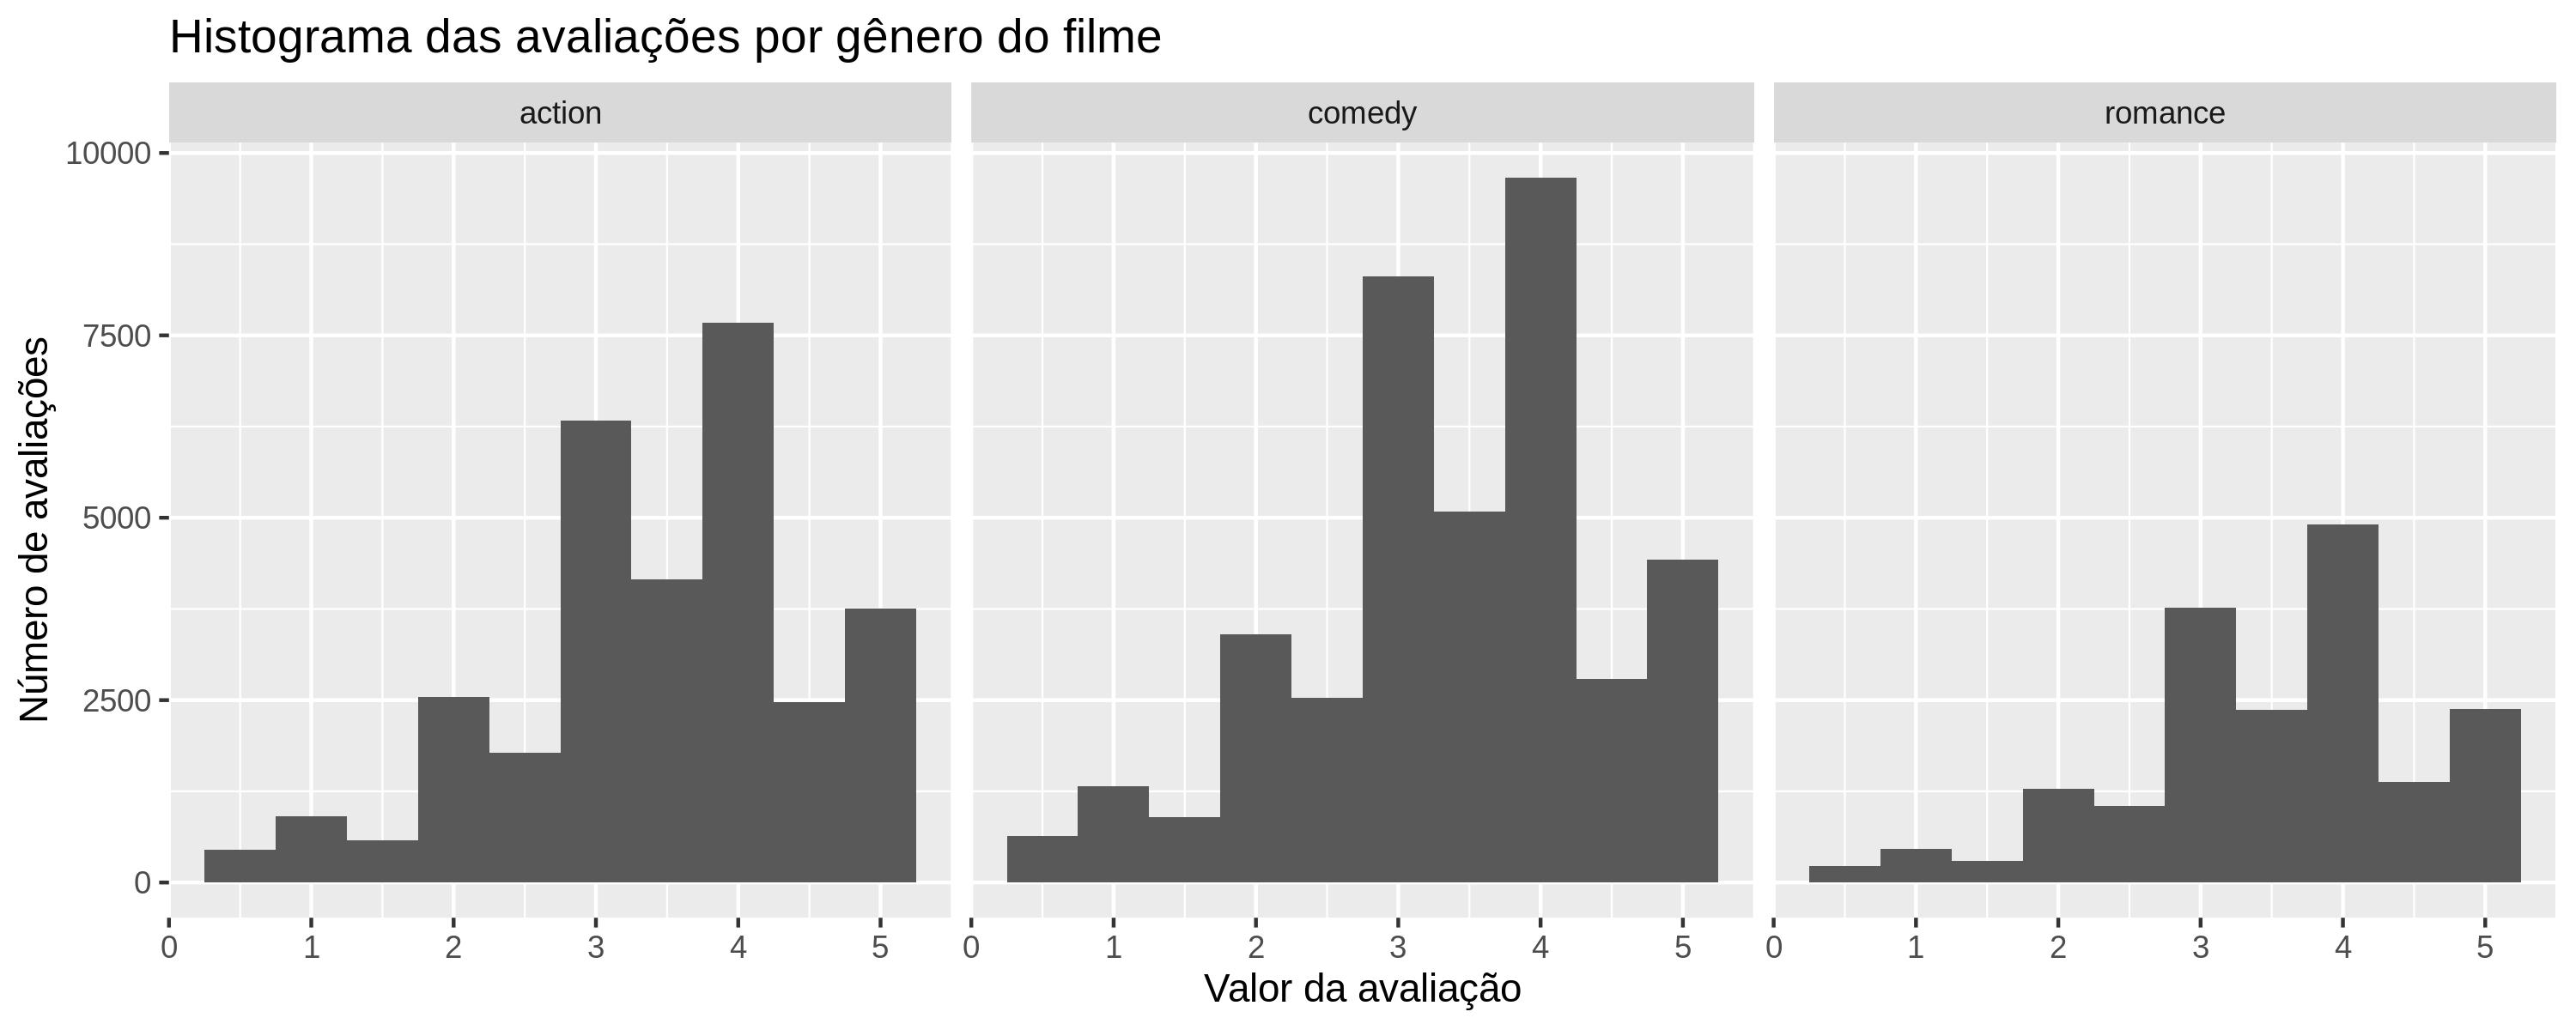
\includegraphics{./histogram.jpg}
\caption{}
\end{figure}

Como podemos observar, a os dados se distribuem de maneira normal
fazendo com que se tornem bons dados para esse tipo de análise.

Ao gerar os intervalos de confiança temos:

\begin{Shaded}
\begin{Highlighting}[]
\NormalTok{  header =}\StringTok{ }\KeywordTok{c}\NormalTok{(}\StringTok{'Romance'}\NormalTok{, }\StringTok{'Action'}\NormalTok{, }\StringTok{'Comedy'}\NormalTok{)}
\NormalTok{  cis =}\StringTok{  }\KeywordTok{data.frame}\NormalTok{(}
            \KeywordTok{CI}\NormalTok{(ratings_romance[[}\StringTok{'rating'}\NormalTok{]], }\DataTypeTok{ci=}\FloatTok{0.95}\NormalTok{),}
            \KeywordTok{CI}\NormalTok{(ratings_action[[}\StringTok{'rating'}\NormalTok{]], }\DataTypeTok{ci=}\FloatTok{0.95}\NormalTok{), }
            \KeywordTok{CI}\NormalTok{(ratings_comedy[[}\StringTok{'rating'}\NormalTok{]], }\DataTypeTok{ci=}\FloatTok{0.95}\NormalTok{)}
\NormalTok{          )  }
  
  \KeywordTok{names}\NormalTok{(cis) =}\StringTok{ }\NormalTok{header}
\NormalTok{  t_cis =}\StringTok{ }\KeywordTok{data.frame}\NormalTok{(}\KeywordTok{t}\NormalTok{(cis))}


\NormalTok{  cis_generos =}\StringTok{ }\KeywordTok{ggplot}\NormalTok{(t_cis, }\KeywordTok{aes}\NormalTok{(}\KeywordTok{rownames}\NormalTok{(t_cis), mean, }\DataTypeTok{ymin=}\NormalTok{lower, }\DataTypeTok{ymax=}\NormalTok{upper)) }\OperatorTok{+}
\StringTok{    }\KeywordTok{geom_errorbar}\NormalTok{() }\OperatorTok{+}
\StringTok{    }\KeywordTok{geom_point}\NormalTok{(}\DataTypeTok{mapping =} \KeywordTok{aes}\NormalTok{(}\KeywordTok{rownames}\NormalTok{(t_cis), }\DataTypeTok{y=}\NormalTok{mean)) }\OperatorTok{+}
\StringTok{    }\KeywordTok{xlab}\NormalTok{(}\StringTok{"Gêneros") + ylab("}\NormalTok{Intervalo de confiança para avaliação média}\StringTok{")}
\StringTok{  ggsave('cis_generos.jpg')}
\end{Highlighting}
\end{Shaded}

\begin{verbatim}
## Saving 6.5 x 4.5 in image
\end{verbatim}

\begin{figure}
\centering
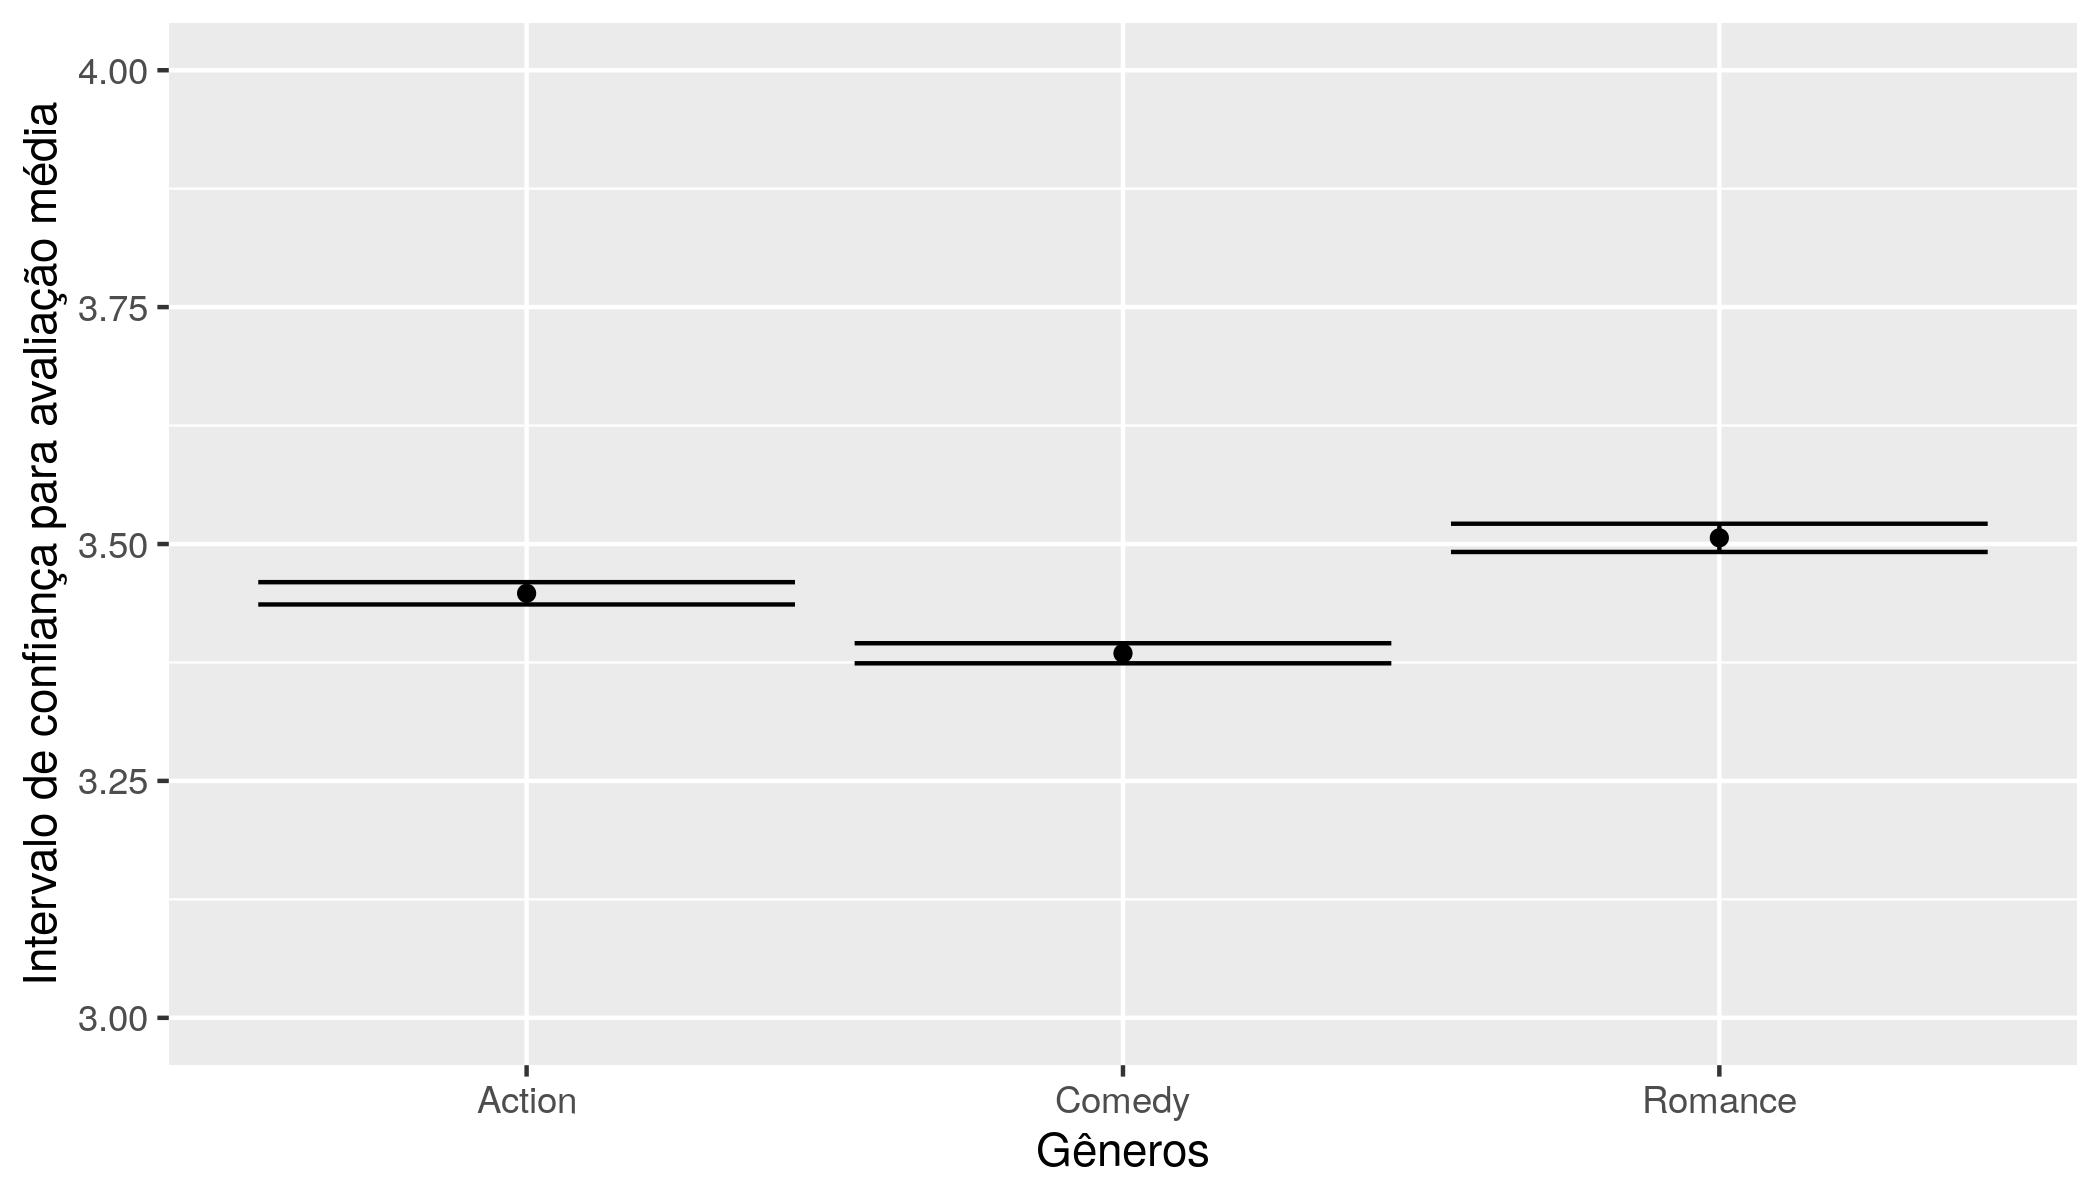
\includegraphics{./cis_generos.jpg}
\caption{}
\end{figure}

\begin{center}\rule{0.5\linewidth}{\linethickness}\end{center}

\paragraph{\texorpdfstring{2. \textbf{\emph{Senhor dos Anéis} vs
\emph{Harry Potter}, algum dos dois é melhor
avaliado?}}{2. Senhor dos Anéis vs Harry Potter, algum dos dois é melhor avaliado?}}\label{senhor-dos-anuxe9is-vs-harry-potter-algum-dos-dois-uxe9-melhor-avaliado}

Para responder essa pergunta iremos fazer um processo similar ao
anterior.

\begin{Shaded}
\begin{Highlighting}[]
\NormalTok{  d =}\StringTok{ }\KeywordTok{bind_rows}\NormalTok{(ratings_lotr, ratings_harry) }\OperatorTok\StringTok{ }\KeywordTok{group_by}\NormalTok{(title) }\OperatorTok\StringTok{ }\KeywordTok{summarise}\NormalTok{(}\DataTypeTok{mean=}\KeywordTok{mean}\NormalTok{(rating), }\DataTypeTok{median=}\KeywordTok{median}\NormalTok{(rating))}
  \KeywordTok{kable}\NormalTok{(d)}
\end{Highlighting}
\end{Shaded}

\begin{longtable}[]{@{}lrr@{}}
\toprule
title & mean & median\tabularnewline
\midrule
\endhead
Harry Potter & 3.817406 & 4\tabularnewline
Lord of the Rings & 4.058020 & 4\tabularnewline
\bottomrule
\end{longtable}

Podemos ver que a mediana e a média seguem comportamento igual a análise
anterior, porém a distância das médias é um pouco maior para esse
subconjunto dos dados.

Gerando o intervalo de confiança temos:

\begin{Shaded}
\begin{Highlighting}[]
\NormalTok{  ci_lotr =}\StringTok{ }\KeywordTok{CI}\NormalTok{(ratings_lotr[[}\StringTok{'rating'}\NormalTok{]], }\DataTypeTok{ci=}\FloatTok{0.95}\NormalTok{)}
\NormalTok{  ci_harry =}\StringTok{ }\KeywordTok{CI}\NormalTok{(ratings_harry[[}\StringTok{'rating'}\NormalTok{]], }\DataTypeTok{ci=}\FloatTok{0.95}\NormalTok{)}
  
\NormalTok{  cis =}\StringTok{ }\KeywordTok{data.frame}\NormalTok{(ci_lotr, ci_harry)}
  \KeywordTok{names}\NormalTok{(cis) =}\StringTok{ }\KeywordTok{c}\NormalTok{(}\StringTok{'Senhor dos Anéis'}\NormalTok{, }\StringTok{'Harry Potter'}\NormalTok{)}
  
\NormalTok{  cis =}\StringTok{ }\KeywordTok{data.frame}\NormalTok{(}\KeywordTok{t}\NormalTok{(cis))}
  
\NormalTok{  var =}\StringTok{ }\KeywordTok{ggplot}\NormalTok{(cis, }\KeywordTok{aes}\NormalTok{(}\KeywordTok{rownames}\NormalTok{(cis), mean, }\DataTypeTok{ymin=}\NormalTok{lower, }\DataTypeTok{ymax=}\NormalTok{upper)) }\OperatorTok{+}
\StringTok{    }\KeywordTok{geom_errorbar}\NormalTok{() }\OperatorTok{+}
\StringTok{    }\KeywordTok{geom_point}\NormalTok{(}\DataTypeTok{mapping =} \KeywordTok{aes}\NormalTok{(}\KeywordTok{rownames}\NormalTok{(cis), }\DataTypeTok{y=}\NormalTok{mean)) }\OperatorTok{+}
\StringTok{    }\KeywordTok{xlab}\NormalTok{(}\StringTok{"Título"}\NormalTok{) }\OperatorTok{+}\StringTok{ }\KeywordTok{ylab}\NormalTok{(}\StringTok{"Intervalo de confiança para avaliação média"}\NormalTok{)}
  \KeywordTok{ggsave}\NormalTok{(}\StringTok{'cis_titulos.jpg'}\NormalTok{)}
\end{Highlighting}
\end{Shaded}

\begin{verbatim}
## Saving 6.5 x 4.5 in image
\end{verbatim}

\begin{figure}
\centering
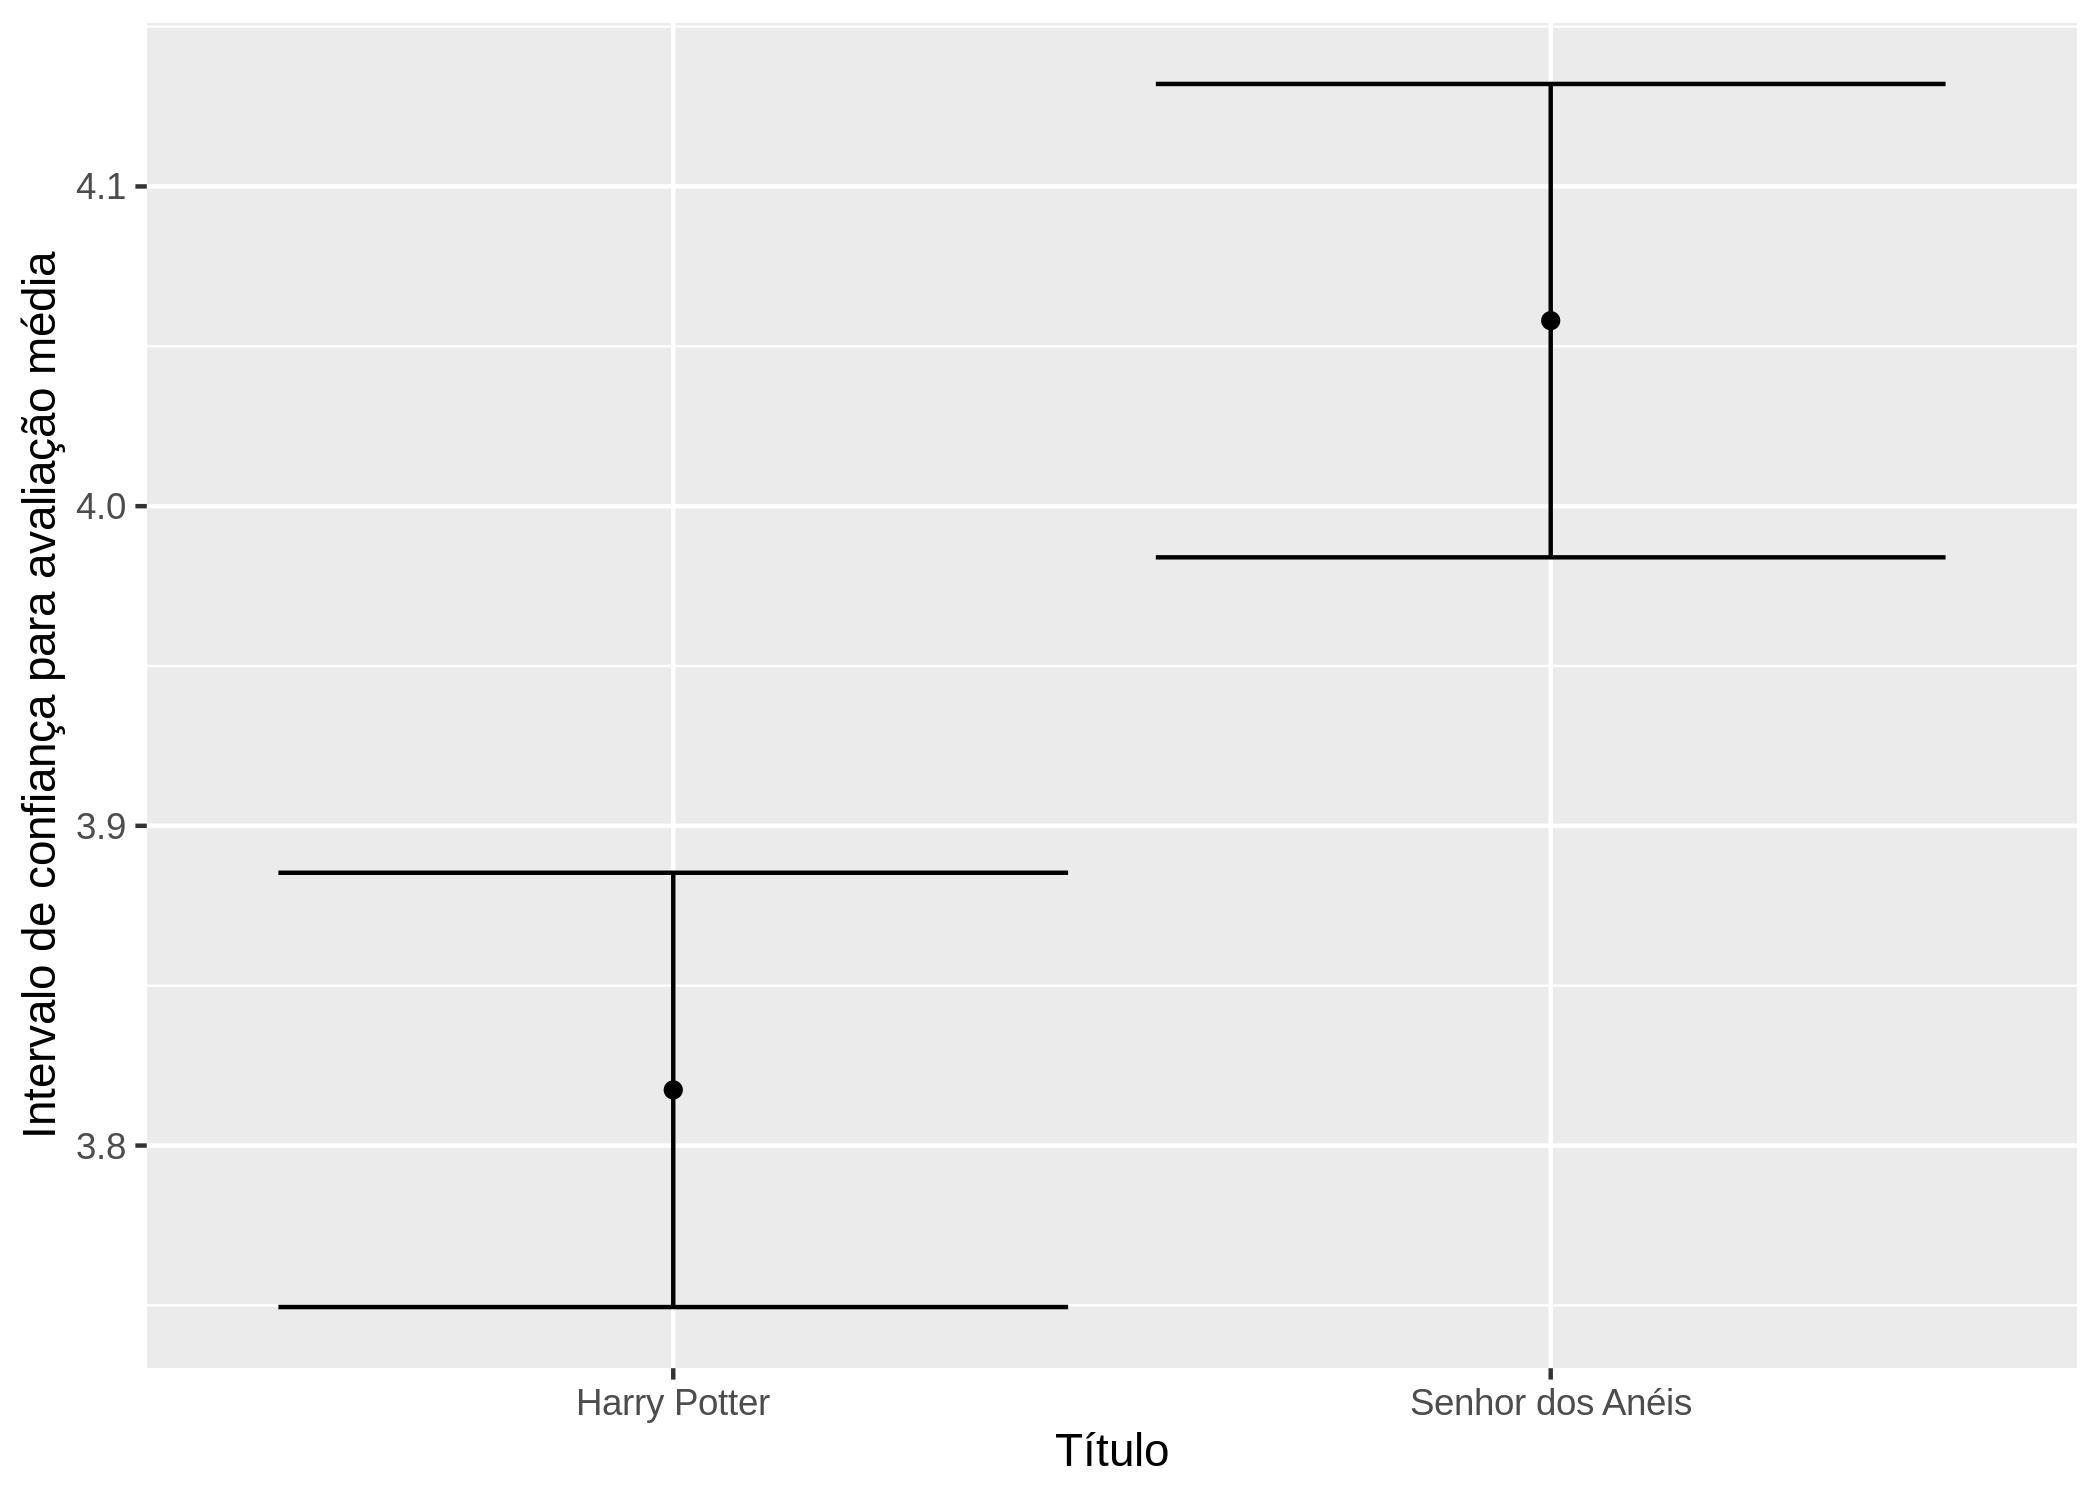
\includegraphics{./cis_titulos.jpg}
\caption{}
\end{figure}

\newpage 

\subsection{Conclusão}\label{conclusuxe3o}

Ao analisar os dados de avaliação desses filmes é difícil fazer
afirmações apenas com medidas como média ou medianas. Principalmente
quando as médias estão muito próximas umas das outras é difícil dizer
que a média de um determinado filme é maior que outra.

Aplicando um intervalo de confiança, com um nível de confiança
relativamente alto nesses dados que apresentam uma distribuição normal
ficamos um pouco mais confortáveis em fazer afirmações sobre a média de
uma amostra da população.

Se considerarmos que a população real, ou seja as opiniões dos
espectadores dos filmes aqui listados, está em concordância com a
amostra que analizamos então outras amostras da população real teriam
resultados próximos aos encontrados.

Na nossa análise pode-se dizer que nossas respostas indicam que:

\begin{enumerate}
\def\labelenumi{\arabic{enumi}.}
\tightlist
\item
  \textbf{Dentre os gêneros de \emph{Ação}, \emph{Romance} e
  \emph{Comédia}; Algum deles recebe avaliação mais alta?}
\end{enumerate}

\begin{itemize}
\tightlist
\item
  Sim, os espectadores deram em média avaliações mais altas para os
  filmes de Romance, Ação e Comédia respectivamente.
\end{itemize}

\begin{enumerate}
\def\labelenumi{\arabic{enumi}.}
\setcounter{enumi}{1}
\tightlist
\item
  \textbf{\emph{Senhor dos Anéis} vs \emph{Harry Potter}, algum dos dois
  é melhor avaliado?}
\end{enumerate}

\begin{itemize}
\tightlist
\item
  Sim, para um intervalo de confiança de 95\% a avaliação média dos
  filmes de \textbf{O Senhor dos Anéis} (3.98 \textasciitilde{} 4.13),
  costuma ser mais alta do que a avaliação média de \textbf{Harry
  Potter} (3.75 \textasciitilde{} 3.88)
\end{itemize}


\end{document}
